\documentclass[twoside]{book}

% Packages required by doxygen
\usepackage{fixltx2e}
\usepackage{calc}
\usepackage{doxygen}
\usepackage[export]{adjustbox} % also loads graphicx
\usepackage{graphicx}
\usepackage[utf8]{inputenc}
\usepackage{makeidx}
\usepackage{multicol}
\usepackage{multirow}
\PassOptionsToPackage{warn}{textcomp}
\usepackage{textcomp}
\usepackage[nointegrals]{wasysym}
\usepackage[table]{xcolor}

% Font selection
\usepackage[T1]{fontenc}
\usepackage[scaled=.90]{helvet}
\usepackage{courier}
\usepackage{amssymb}
\usepackage{sectsty}
\renewcommand{\familydefault}{\sfdefault}
\allsectionsfont{%
  \fontseries{bc}\selectfont%
  \color{darkgray}%
}
\renewcommand{\DoxyLabelFont}{%
  \fontseries{bc}\selectfont%
  \color{darkgray}%
}
\newcommand{\+}{\discretionary{\mbox{\scriptsize$\hookleftarrow$}}{}{}}

% Page & text layout
\usepackage{geometry}
\geometry{%
  a4paper,%
  top=2.5cm,%
  bottom=2.5cm,%
  left=2.5cm,%
  right=2.5cm%
}
\tolerance=750
\hfuzz=15pt
\hbadness=750
\setlength{\emergencystretch}{15pt}
\setlength{\parindent}{0cm}
\setlength{\parskip}{3ex plus 2ex minus 2ex}
\makeatletter
\renewcommand{\paragraph}{%
  \@startsection{paragraph}{4}{0ex}{-1.0ex}{1.0ex}{%
    \normalfont\normalsize\bfseries\SS@parafont%
  }%
}
\renewcommand{\subparagraph}{%
  \@startsection{subparagraph}{5}{0ex}{-1.0ex}{1.0ex}{%
    \normalfont\normalsize\bfseries\SS@subparafont%
  }%
}
\makeatother

% Headers & footers
\usepackage{fancyhdr}
\pagestyle{fancyplain}
\fancyhead[LE]{\fancyplain{}{\bfseries\thepage}}
\fancyhead[CE]{\fancyplain{}{}}
\fancyhead[RE]{\fancyplain{}{\bfseries\leftmark}}
\fancyhead[LO]{\fancyplain{}{\bfseries\rightmark}}
\fancyhead[CO]{\fancyplain{}{}}
\fancyhead[RO]{\fancyplain{}{\bfseries\thepage}}
\fancyfoot[LE]{\fancyplain{}{}}
\fancyfoot[CE]{\fancyplain{}{}}
\fancyfoot[RE]{\fancyplain{}{\bfseries\scriptsize Generated by Doxygen }}
\fancyfoot[LO]{\fancyplain{}{\bfseries\scriptsize Generated by Doxygen }}
\fancyfoot[CO]{\fancyplain{}{}}
\fancyfoot[RO]{\fancyplain{}{}}
\renewcommand{\footrulewidth}{0.4pt}
\renewcommand{\chaptermark}[1]{%
  \markboth{#1}{}%
}
\renewcommand{\sectionmark}[1]{%
  \markright{\thesection\ #1}%
}

% Indices & bibliography
\usepackage{natbib}
\usepackage[titles]{tocloft}
\setcounter{tocdepth}{3}
\setcounter{secnumdepth}{5}
\makeindex

% Hyperlinks (required, but should be loaded last)
\usepackage{ifpdf}
\ifpdf
  \usepackage[pdftex,pagebackref=true]{hyperref}
\else
  \usepackage[ps2pdf,pagebackref=true]{hyperref}
\fi
\hypersetup{%
  colorlinks=true,%
  linkcolor=blue,%
  citecolor=blue,%
  unicode%
}

% Custom commands
\newcommand{\clearemptydoublepage}{%
  \newpage{\pagestyle{empty}\cleardoublepage}%
}

\usepackage{caption}
\captionsetup{labelsep=space,justification=centering,font={bf},singlelinecheck=off,skip=4pt,position=top}

%===== C O N T E N T S =====

\begin{document}

% Titlepage & ToC
\hypersetup{pageanchor=false,
             bookmarksnumbered=true,
             pdfencoding=unicode
            }
\pagenumbering{alph}
\begin{titlepage}
\vspace*{7cm}
\begin{center}%
{\Large Haptic Vision (H\+Viz) \\[1ex]\large v1.\+0.\+0 }\\
\vspace*{1cm}
{\large Generated by Doxygen 1.8.13}\\
\end{center}
\end{titlepage}
\clearemptydoublepage
\pagenumbering{roman}
\tableofcontents
\clearemptydoublepage
\pagenumbering{arabic}
\hypersetup{pageanchor=true}

%--- Begin generated contents ---
\chapter{Requirements}
\label{index}\hypertarget{index}{}A device that helps perceive your surrounding by using the sense of touch with deployment of Y\+O\+L\+Ov5 through Lib\+Torch C++ A\+PI.

\section*{Requirements}


\begin{DoxyItemize}
\item \href{https://www.instructables.com/Install-Ubuntu-18044-LTS-on-Your-Raspberry-Pi-Boar/}{\tt Ubuntu 18.\+04}
\item Open\+CV 3.\+2.\+0
\item \href{https://download.pytorch.org/libtorch/nightly/cpu/libtorch-shared-with-deps-latest.zip}{\tt Lib\+Torch 1.\+6.\+0}
\item \href{https://askubuntu.com/questions/355565/how-do-i-install-the-latest-version-of-cmake-from-the-command-line}{\tt C\+Make 3.\+10.\+2}
\item \href{https://abyz.me.uk/rpi/pigpio/download.html}{\tt pi\+G\+P\+IO}
\end{DoxyItemize}

\section*{Software-\/stack}

To setup and run the device use the following steps\+:

\subsection*{To run}


\begin{DoxyEnumerate}
\item Update raspberry pi 
\begin{DoxyCode}
sudo apt update
sudo apt upgrade
\end{DoxyCode}

\item Install pigpio 
\begin{DoxyCode}
sudo apt-get install libpigpio-dev
\end{DoxyCode}

\item Install Qt 
\begin{DoxyCode}
sudo apt-get install qtdeclarative5-dev-tools
sudo apt-get install libqwt-qt5-dev
\end{DoxyCode}

\item Install Open\+CV 
\begin{DoxyCode}
sudo apt install libopencv-dev
sudo apt install libopencv-core-dev
\end{DoxyCode}

\item Setup Pi Cam Once the ribbon cable is connected to the rasperry pi. Got to raspberry pi configurator 
\begin{DoxyCode}
sudo raspi-config
\end{DoxyCode}

\item Go to interface and enable camera option. Then restart you Pi.
\item Once Pi is restarted, check of camera is working by 
\begin{DoxyCode}
libcamera-jpeg -o image.jpg
\end{DoxyCode}

\item If raspicam dependencies are not installed, follow steps in the following \href{https://github.com/cedricve/raspicam}{\tt link}.
\item Clone program files onto the rasperry pi.
\item Compile and run. 
\begin{DoxyCode}
mkdir build && cd build
cmake ..
make
./../bin/HViz\_run
\end{DoxyCode}

\end{DoxyEnumerate}

Note\+:
\begin{DoxyItemize}
\item Libtorch package solely contributes to the presence of python files in the project.
\item C\+O\+C\+O-\/pretrained Y\+O\+L\+Ov5s model has been provided. For more pretrained models, see \href{https://github.com/ultralytics/yolov5}{\tt yolov5}.
\end{DoxyItemize}

\section*{Technologies}

H\+Viz is built using\+:


\begin{DoxyItemize}
\item \href{https://www.cplusplus.com/}{\tt C++ Programming Language}
\item \href{https://www.linux.org/}{\tt Debian/\+Ubuntu Linux}
\item \href{https://www.raspberrypi.org}{\tt Raspberry Pi}
\item \href{https://cmake.org/}{\tt Cmake}
\item \href{https://opencv.org/}{\tt Open\+CV}
\item \href{https://github.com/google/googletest}{\tt Google Test}
\item \href{https://www.doxygen.nl/index.html}{\tt Doxygen}
\item \href{https://www.qt.io/}{\tt Qt}
\end{DoxyItemize}

\subsection*{Socials}


\begin{DoxyItemize}
\item \href{https://www.instagram.com/hapticvision_/}{\tt Instagram}
\end{DoxyItemize}

\subsection*{The Team}


\begin{DoxyItemize}
\item \href{https://github.com/rdj2829}{\tt rdj2829}
\item \href{https://github.com/dheerajsankar}{\tt dheerajsankar}
\item \href{https://github.com/kprakz}{\tt kprakz}
\item \href{https://github.com/josephjoel3099}{\tt josephjoel3099}
\end{DoxyItemize}

\subsection*{Contact Us}


\begin{DoxyItemize}
\item DM us on \href{https://www.instagram.com/hapticvision_/}{\tt hapticvision\+\_\+}
\item Email us at \href{mailto:hapticvisionuofg@gmail.com}{\tt hapticvisionuofg@gmail.\+com} 
\end{DoxyItemize}
\chapter{C\+AD files}
\label{md__home_joseph_hviz_joel_ss_extras_CAD_files_README}
\Hypertarget{md__home_joseph_hviz_joel_ss_extras_CAD_files_README}
C\+AD files here 
\chapter{Documentation}
\label{md__home_joseph_hviz_joel_ss_extras_Documentation_README}
\Hypertarget{md__home_joseph_hviz_joel_ss_extras_Documentation_README}
All images, docs and P\+P\+Ts made for the project are here 
\chapter{Electronics}
\label{md__home_joseph_hviz_joel_ss_extras_Electronics_README}
\Hypertarget{md__home_joseph_hviz_joel_ss_extras_Electronics_README}
All P\+CB designs, electronics and related stuff here

 
\chapter{Haptic\+Vision (aka \char`\"{}\+H\+Viz\char`\"{})}
\label{md__home_joseph_hviz_joel_ss_extras_General_README}
\Hypertarget{md__home_joseph_hviz_joel_ss_extras_General_README}
A device that helps perceive your surrounding by using the sense of touch.



\subsection*{The Team}


\begin{DoxyItemize}
\item \href{https://github.com/rdj2829}{\tt }
\item \href{https://github.com/dheerajsankar}{\tt }
\item \href{https://github.com/kprakz}{\tt }
\item \href{https://github.com/josephjoel3099}{\tt }
\end{DoxyItemize}

\subsection*{Socials}


\begin{DoxyItemize}
\item \href{https://www.instagram.com/hapticvision_/}{\tt Instagram}
\end{DoxyItemize}

\subsection*{Repos}


\begin{DoxyItemize}
\item \href{https://github.com/Haptic-Vision/Documentation}{\tt Documentation}
\item \href{https://github.com/Haptic-Vision/Socials}{\tt Socials}
\item \href{https://github.com/Haptic-Vision/Housekeeping}{\tt Housekeeping}
\item \href{https://github.com/Haptic-Vision/Electronics}{\tt Electronics}
\item \href{https://github.com/Haptic-Vision/Software-stack}{\tt Software-\/stack} 
\end{DoxyItemize}
\chapter{Housekeeping}
\label{md__home_joseph_hviz_joel_ss_extras_Housekeeping_README}
\Hypertarget{md__home_joseph_hviz_joel_ss_extras_Housekeeping_README}
Material list, Work allocation and related docs are here 
\chapter{Socials}
\label{md__home_joseph_hviz_joel_ss_extras_Socials_README}
\Hypertarget{md__home_joseph_hviz_joel_ss_extras_Socials_README}
All images, videos and related stuff for socials here 
\chapter{Haptic\+Vision (aka \char`\"{}\+H\+Viz\char`\"{})}
\label{md__home_joseph_hviz_joel_ss_README}
\Hypertarget{md__home_joseph_hviz_joel_ss_README}
A device that helps perceive your surrounding by using the sense of touch with deployment of Y\+O\+L\+Ov5 through Lib\+Torch C++ A\+PI.



   \href{https://github.com/Haptic-Vision/haptic_vision/blob/main/LICENSE}{\tt } ~\newline
 \href{https://github.com/MataPOS/matapos/issues}{\tt Report Bug} \href{https://github.com/MataPOS/matapos/issues}{\tt Request Feature} ~\newline


 

\section*{Requirements}


\begin{DoxyItemize}
\item \href{https://www.instructables.com/Install-Ubuntu-18044-LTS-on-Your-Raspberry-Pi-Boar/}{\tt Ubuntu 18.\+04}
\item Open\+CV 3.\+2.\+0
\item \href{https://download.pytorch.org/libtorch/nightly/cpu/libtorch-shared-with-deps-latest.zip}{\tt Lib\+Torch 1.\+6.\+0}
\item \href{https://askubuntu.com/questions/355565/how-do-i-install-the-latest-version-of-cmake-from-the-command-line}{\tt C\+Make 3.\+10.\+2}
\item \href{https://abyz.me.uk/rpi/pigpio/download.html}{\tt pi\+G\+P\+IO}
\end{DoxyItemize}

\section*{Software-\/stack}

To setup and run the device use the following steps\+:



\subsection*{To run}


\begin{DoxyEnumerate}
\item Update raspberry pi 
\begin{DoxyCode}
sudo apt update
sudo apt upgrade
\end{DoxyCode}

\item Install pigpio 
\begin{DoxyCode}
sudo apt-get install libpigpio-dev
\end{DoxyCode}

\item Install Qt 
\begin{DoxyCode}
sudo apt-get install qtdeclarative5-dev-tools
sudo apt-get install libqwt-qt5-dev
\end{DoxyCode}

\item Install Open\+CV 
\begin{DoxyCode}
sudo apt install libopencv-dev
sudo apt install libopencv-core-dev
\end{DoxyCode}

\item Setup Pi Cam Once the ribbon cable is connected to the rasperry pi. Got to raspberry pi configurator 
\begin{DoxyCode}
sudo raspi-config
\end{DoxyCode}

\item Go to interface and enable camera option. Then restart you Pi.
\item Once Pi is restarted, check of camera is working by 
\begin{DoxyCode}
libcamera-jpeg -o image.jpg
\end{DoxyCode}

\item If raspicam dependencies are not installed, follow steps in the following \href{https://github.com/cedricve/raspicam}{\tt link}.
\item Clone program files onto the rasperry pi.
\item Compile and run. 
\begin{DoxyCode}
mkdir build && cd build
cmake ..
make
./../bin/HViz\_run
\end{DoxyCode}

\end{DoxyEnumerate}

Note\+:
\begin{DoxyItemize}
\item Libtorch package solely contributes to the presence of python files in the project.
\item C\+O\+C\+O-\/pretrained Y\+O\+L\+Ov5s model has been provided. For more pretrained models, see \href{https://github.com/ultralytics/yolov5}{\tt yolov5}.
\end{DoxyItemize}

\section*{Circuit Design}



\section*{Technologies}

H\+Viz is built using\+:


\begin{DoxyItemize}
\item \href{https://www.cplusplus.com/}{\tt C++ Programming Language}
\item \href{https://www.linux.org/}{\tt Debian/\+Ubuntu Linux}
\item \href{https://www.raspberrypi.org}{\tt Raspberry Pi}
\item \href{https://cmake.org/}{\tt Cmake}
\item \href{https://opencv.org/}{\tt Open\+CV}
\item \href{https://github.com/google/googletest}{\tt Google Test}
\item \href{https://www.doxygen.nl/index.html}{\tt Doxygen}
\item \href{https://www.qt.io/}{\tt Qt}
\end{DoxyItemize}

\subsection*{Socials}

\href{https://www.instagram.com/hapticvision_/}{\tt }


\begin{DoxyItemize}
\item \href{https://www.instagram.com/hapticvision_/}{\tt Instagram}
\end{DoxyItemize}

\subsection*{The Team}


\begin{DoxyItemize}
\item \href{https://github.com/rdj2829}{\tt }
\item \href{https://github.com/dheerajsankar}{\tt }
\item \href{https://github.com/kprakz}{\tt }
\item \href{https://github.com/josephjoel3099}{\tt }
\end{DoxyItemize}

\subsection*{Contact Us}


\begin{DoxyItemize}
\item DM us on \href{https://www.instagram.com/hapticvision_/}{\tt }
\item Email us at $\ast$$\ast$hapticvisionuofg.com$\ast$$\ast$
\end{DoxyItemize}

\subsection*{License}
\chapter{Class Index}
\section{Class List}
Here are the classes, structs, unions and interfaces with brief descriptions\+:\begin{DoxyCompactList}
\item\contentsline{section}{\hyperlink{classCameraCapture}{Camera\+Capture} }{\pageref{classCameraCapture}}{}
\item\contentsline{section}{\hyperlink{classGPIOController}{G\+P\+I\+O\+Controller} }{\pageref{classGPIOController}}{}
\item\contentsline{section}{\hyperlink{classObstacleDetector}{Obstacle\+Detector} }{\pageref{classObstacleDetector}}{}
\item\contentsline{section}{\hyperlink{classYolo}{Yolo} }{\pageref{classYolo}}{}
\end{DoxyCompactList}

\chapter{File Index}
\section{File List}
Here is a list of all documented files with brief descriptions\+:\begin{DoxyCompactList}
\item\contentsline{section}{/home/joseph/hviz\+\_\+joel\+\_\+ss/lib/camera/\hyperlink{CameraCapture_8cpp}{Camera\+Capture.\+cpp} \\*This files defines all the function needed to run the camera }{\pageref{CameraCapture_8cpp}}{}
\item\contentsline{section}{/home/joseph/hviz\+\_\+joel\+\_\+ss/lib/camera/\hyperlink{CameraCapture_8h}{Camera\+Capture.\+h} \\*The file declares all the headers and functions for running the camera }{\pageref{CameraCapture_8h}}{}
\item\contentsline{section}{/home/joseph/hviz\+\_\+joel\+\_\+ss/lib/gpio\+\_\+controller/\hyperlink{GPIOController_8cpp}{G\+P\+I\+O\+Controller.\+cpp} \\*Contains all the function needed to actuate the motors on the gloves }{\pageref{GPIOController_8cpp}}{}
\item\contentsline{section}{/home/joseph/hviz\+\_\+joel\+\_\+ss/lib/gpio\+\_\+controller/\hyperlink{GPIOController_8h}{G\+P\+I\+O\+Controller.\+h} \\*The file declares all the headers and functions to actuate the motors on the gloves }{\pageref{GPIOController_8h}}{}
\item\contentsline{section}{/home/joseph/hviz\+\_\+joel\+\_\+ss/lib/obstacle\+\_\+detector/\hyperlink{ObstacleDetector_8cpp}{Obstacle\+Detector.\+cpp} \\*Code to detect and read out position of obstacle }{\pageref{ObstacleDetector_8cpp}}{}
\item\contentsline{section}{/home/joseph/hviz\+\_\+joel\+\_\+ss/lib/obstacle\+\_\+detector/\hyperlink{ObstacleDetector_8h}{Obstacle\+Detector.\+h} \\*The file declares all the headers and functions to detct position of obstacle }{\pageref{ObstacleDetector_8h}}{}
\item\contentsline{section}{/home/joseph/hviz\+\_\+joel\+\_\+ss/lib/yolo/\hyperlink{Yolo_8cpp}{Yolo.\+cpp} \\*Contains all the definitions of functions need for object detection using Y\+O\+LO }{\pageref{Yolo_8cpp}}{}
\item\contentsline{section}{/home/joseph/hviz\+\_\+joel\+\_\+ss/lib/yolo/\hyperlink{Yolo_8h}{Yolo.\+h} \\*This file declares all the headers and functions needed for Y\+O\+LO object detection and clasiffication }{\pageref{Yolo_8h}}{}
\item\contentsline{section}{/home/joseph/hviz\+\_\+joel\+\_\+ss/src/\hyperlink{main_8cpp}{main.\+cpp} \\*This file is the main code to run the system }{\pageref{main_8cpp}}{}
\end{DoxyCompactList}

\chapter{Class Documentation}
\hypertarget{classCameraCapture}{}\section{Camera\+Capture Class Reference}
\label{classCameraCapture}\index{Camera\+Capture@{Camera\+Capture}}
\subsection*{Public Member Functions}
\begin{DoxyCompactItemize}
\item 
\mbox{\Hypertarget{classCameraCapture_a9dfe4e4bc8dcf369977e6e81f4f438b1}\label{classCameraCapture_a9dfe4e4bc8dcf369977e6e81f4f438b1}} 
\hyperlink{classCameraCapture_a9dfe4e4bc8dcf369977e6e81f4f438b1}{Camera\+Capture} ()
\begin{DoxyCompactList}\small\item\em Construct a new Camera Capture\+:\+: Camera Capture object. \end{DoxyCompactList}\item 
\mbox{\Hypertarget{classCameraCapture_a9fb9058c34d463b8bf9055b2f129adac}\label{classCameraCapture_a9fb9058c34d463b8bf9055b2f129adac}} 
\hyperlink{classCameraCapture_a9fb9058c34d463b8bf9055b2f129adac}{$\sim$\+Camera\+Capture} ()
\begin{DoxyCompactList}\small\item\em Destroy the Camera Capture\+:\+: Camera Capture object. \end{DoxyCompactList}\item 
bool \hyperlink{classCameraCapture_a1a0212fc06b71d35e613b3c781f0814b}{open} (int index)
\begin{DoxyCompactList}\small\item\em Function opens the launches the camera and gives feedback of its state. \end{DoxyCompactList}\item 
\mbox{\Hypertarget{classCameraCapture_a452aa68c9cf0f1c46586af54faee7bfe}\label{classCameraCapture_a452aa68c9cf0f1c46586af54faee7bfe}} 
void \hyperlink{classCameraCapture_a452aa68c9cf0f1c46586af54faee7bfe}{close} ()
\begin{DoxyCompactList}\small\item\em Function closes the camera. \end{DoxyCompactList}\item 
bool \hyperlink{classCameraCapture_af7fbe43ef6352fae2ca2458a60cd8b9f}{is\+Opened} () const
\begin{DoxyCompactList}\small\item\em Checks if camera is open. \end{DoxyCompactList}\item 
bool \hyperlink{classCameraCapture_a3a1d86aca613881d8cd06d3f7b85440f}{read} (cv\+::\+Mat \&frame)
\begin{DoxyCompactList}\small\item\em Records data from camera. \end{DoxyCompactList}\item 
void \hyperlink{classCameraCapture_af82994a1857ad331f8d9d24b3ae24962}{set\+Property} (int prop\+Id, double value)
\begin{DoxyCompactList}\small\item\em Used to set camera properties. \end{DoxyCompactList}\end{DoxyCompactItemize}


\subsection{Member Function Documentation}
\mbox{\Hypertarget{classCameraCapture_af7fbe43ef6352fae2ca2458a60cd8b9f}\label{classCameraCapture_af7fbe43ef6352fae2ca2458a60cd8b9f}} 
\index{Camera\+Capture@{Camera\+Capture}!is\+Opened@{is\+Opened}}
\index{is\+Opened@{is\+Opened}!Camera\+Capture@{Camera\+Capture}}
\subsubsection{\texorpdfstring{is\+Opened()}{isOpened()}}
{\footnotesize\ttfamily bool Camera\+Capture\+::is\+Opened (\begin{DoxyParamCaption}{ }\end{DoxyParamCaption}) const}



Checks if camera is open. 

\begin{DoxyReturn}{Returns}
true 

false 
\end{DoxyReturn}
\mbox{\Hypertarget{classCameraCapture_a1a0212fc06b71d35e613b3c781f0814b}\label{classCameraCapture_a1a0212fc06b71d35e613b3c781f0814b}} 
\index{Camera\+Capture@{Camera\+Capture}!open@{open}}
\index{open@{open}!Camera\+Capture@{Camera\+Capture}}
\subsubsection{\texorpdfstring{open()}{open()}}
{\footnotesize\ttfamily bool Camera\+Capture\+::open (\begin{DoxyParamCaption}\item[{int}]{index }\end{DoxyParamCaption})}



Function opens the launches the camera and gives feedback of its state. 


\begin{DoxyParams}{Parameters}
{\em index} & \\
\hline
\end{DoxyParams}
\begin{DoxyReturn}{Returns}
true 

false 
\end{DoxyReturn}
\mbox{\Hypertarget{classCameraCapture_a3a1d86aca613881d8cd06d3f7b85440f}\label{classCameraCapture_a3a1d86aca613881d8cd06d3f7b85440f}} 
\index{Camera\+Capture@{Camera\+Capture}!read@{read}}
\index{read@{read}!Camera\+Capture@{Camera\+Capture}}
\subsubsection{\texorpdfstring{read()}{read()}}
{\footnotesize\ttfamily bool Camera\+Capture\+::read (\begin{DoxyParamCaption}\item[{cv\+::\+Mat \&}]{frame }\end{DoxyParamCaption})}



Records data from camera. 


\begin{DoxyParams}{Parameters}
{\em frame} & \\
\hline
\end{DoxyParams}
\begin{DoxyReturn}{Returns}
true 

false 
\end{DoxyReturn}
\mbox{\Hypertarget{classCameraCapture_af82994a1857ad331f8d9d24b3ae24962}\label{classCameraCapture_af82994a1857ad331f8d9d24b3ae24962}} 
\index{Camera\+Capture@{Camera\+Capture}!set\+Property@{set\+Property}}
\index{set\+Property@{set\+Property}!Camera\+Capture@{Camera\+Capture}}
\subsubsection{\texorpdfstring{set\+Property()}{setProperty()}}
{\footnotesize\ttfamily void Camera\+Capture\+::set\+Property (\begin{DoxyParamCaption}\item[{int}]{prop\+Id,  }\item[{double}]{value }\end{DoxyParamCaption})}



Used to set camera properties. 


\begin{DoxyParams}{Parameters}
{\em prop\+Id} & \\
\hline
{\em value} & \\
\hline
\end{DoxyParams}


The documentation for this class was generated from the following files\+:\begin{DoxyCompactItemize}
\item 
/home/joseph/hviz\+\_\+joel\+\_\+ss/lib/camera/\hyperlink{CameraCapture_8h}{Camera\+Capture.\+h}\item 
/home/joseph/hviz\+\_\+joel\+\_\+ss/lib/camera/\hyperlink{CameraCapture_8cpp}{Camera\+Capture.\+cpp}\end{DoxyCompactItemize}

\hypertarget{classGPIOController}{}\section{G\+P\+I\+O\+Controller Class Reference}
\label{classGPIOController}\index{G\+P\+I\+O\+Controller@{G\+P\+I\+O\+Controller}}
\subsection*{Public Member Functions}
\begin{DoxyCompactItemize}
\item 
\mbox{\Hypertarget{classGPIOController_a4d8d168fd28a39588bb4f0cbbc4a9c68}\label{classGPIOController_a4d8d168fd28a39588bb4f0cbbc4a9c68}} 
\hyperlink{classGPIOController_a4d8d168fd28a39588bb4f0cbbc4a9c68}{G\+P\+I\+O\+Controller} ()
\begin{DoxyCompactList}\small\item\em Construct a new \hyperlink{classGPIOController_a4d8d168fd28a39588bb4f0cbbc4a9c68}{G\+P\+I\+O\+Controller\+::\+G\+P\+I\+O\+Controller} object. \end{DoxyCompactList}\item 
\mbox{\Hypertarget{classGPIOController_aa70ab5fdd57d971ce87a59b7df678c39}\label{classGPIOController_aa70ab5fdd57d971ce87a59b7df678c39}} 
\hyperlink{classGPIOController_aa70ab5fdd57d971ce87a59b7df678c39}{$\sim$\+G\+P\+I\+O\+Controller} ()
\begin{DoxyCompactList}\small\item\em Destroy the \hyperlink{classGPIOController_a4d8d168fd28a39588bb4f0cbbc4a9c68}{G\+P\+I\+O\+Controller\+::\+G\+P\+I\+O\+Controller} object. \end{DoxyCompactList}\item 
void \hyperlink{classGPIOController_a3ed1cb3ef1e79636604c9eb24b1eada6}{setup\+Pin} (int pin\+Number, int mode)
\begin{DoxyCompactList}\small\item\em The functions sets the pins mode. \end{DoxyCompactList}\item 
void \hyperlink{classGPIOController_afec1b6d1415900dc1f99050a471b9f50}{write\+Pin} (int pin\+Number, int value)
\begin{DoxyCompactList}\small\item\em This functions sets the pin to H\+I\+GH or L\+OW. \end{DoxyCompactList}\item 
int \hyperlink{classGPIOController_a90288cf1fa64c2e00e9b7ecfc35dbd54}{read\+Pin} (int pin\+Number)
\begin{DoxyCompactList}\small\item\em This function reads the pin\textquotesingle{}s state. \end{DoxyCompactList}\end{DoxyCompactItemize}


\subsection{Member Function Documentation}
\mbox{\Hypertarget{classGPIOController_a90288cf1fa64c2e00e9b7ecfc35dbd54}\label{classGPIOController_a90288cf1fa64c2e00e9b7ecfc35dbd54}} 
\index{G\+P\+I\+O\+Controller@{G\+P\+I\+O\+Controller}!read\+Pin@{read\+Pin}}
\index{read\+Pin@{read\+Pin}!G\+P\+I\+O\+Controller@{G\+P\+I\+O\+Controller}}
\subsubsection{\texorpdfstring{read\+Pin()}{readPin()}}
{\footnotesize\ttfamily int G\+P\+I\+O\+Controller\+::read\+Pin (\begin{DoxyParamCaption}\item[{int}]{pin\+Number }\end{DoxyParamCaption})}



This function reads the pin\textquotesingle{}s state. 


\begin{DoxyParams}{Parameters}
{\em pin\+Number} & \\
\hline
\end{DoxyParams}
\begin{DoxyReturn}{Returns}
int 
\end{DoxyReturn}
\mbox{\Hypertarget{classGPIOController_a3ed1cb3ef1e79636604c9eb24b1eada6}\label{classGPIOController_a3ed1cb3ef1e79636604c9eb24b1eada6}} 
\index{G\+P\+I\+O\+Controller@{G\+P\+I\+O\+Controller}!setup\+Pin@{setup\+Pin}}
\index{setup\+Pin@{setup\+Pin}!G\+P\+I\+O\+Controller@{G\+P\+I\+O\+Controller}}
\subsubsection{\texorpdfstring{setup\+Pin()}{setupPin()}}
{\footnotesize\ttfamily void G\+P\+I\+O\+Controller\+::setup\+Pin (\begin{DoxyParamCaption}\item[{int}]{pin\+Number,  }\item[{int}]{mode }\end{DoxyParamCaption})}



The functions sets the pins mode. 


\begin{DoxyParams}{Parameters}
{\em pin\+Number} & \\
\hline
{\em mode} & \\
\hline
\end{DoxyParams}
\mbox{\Hypertarget{classGPIOController_afec1b6d1415900dc1f99050a471b9f50}\label{classGPIOController_afec1b6d1415900dc1f99050a471b9f50}} 
\index{G\+P\+I\+O\+Controller@{G\+P\+I\+O\+Controller}!write\+Pin@{write\+Pin}}
\index{write\+Pin@{write\+Pin}!G\+P\+I\+O\+Controller@{G\+P\+I\+O\+Controller}}
\subsubsection{\texorpdfstring{write\+Pin()}{writePin()}}
{\footnotesize\ttfamily void G\+P\+I\+O\+Controller\+::write\+Pin (\begin{DoxyParamCaption}\item[{int}]{pin\+Number,  }\item[{int}]{value }\end{DoxyParamCaption})}



This functions sets the pin to H\+I\+GH or L\+OW. 


\begin{DoxyParams}{Parameters}
{\em pin\+Number} & \\
\hline
{\em value} & \\
\hline
\end{DoxyParams}


The documentation for this class was generated from the following files\+:\begin{DoxyCompactItemize}
\item 
/home/joseph/hviz\+\_\+joel\+\_\+ss/lib/gpio\+\_\+controller/\hyperlink{GPIOController_8h}{G\+P\+I\+O\+Controller.\+h}\item 
/home/joseph/hviz\+\_\+joel\+\_\+ss/lib/gpio\+\_\+controller/\hyperlink{GPIOController_8cpp}{G\+P\+I\+O\+Controller.\+cpp}\end{DoxyCompactItemize}

\hypertarget{classObstacleDetector}{}\section{Obstacle\+Detector Class Reference}
\label{classObstacleDetector}\index{Obstacle\+Detector@{Obstacle\+Detector}}
\subsection*{Public Member Functions}
\begin{DoxyCompactItemize}
\item 
\hyperlink{classObstacleDetector_a48e45d1d34c72092ea9b13b81886342c}{Obstacle\+Detector} (const std\+::string \&model\+Path, const std\+::string \&class\+Names\+Path)
\begin{DoxyCompactList}\small\item\em Construct a new Obstacle Detector\+:\+: Obstacle Detector object. \end{DoxyCompactList}\item 
\mbox{\Hypertarget{classObstacleDetector_a2ecde56ab4f7e9cd0e600b53401da404}\label{classObstacleDetector_a2ecde56ab4f7e9cd0e600b53401da404}} 
void \hyperlink{classObstacleDetector_a2ecde56ab4f7e9cd0e600b53401da404}{process\+Frames} ()
\begin{DoxyCompactList}\small\item\em Main code that prints out the position of the obstacle (Left $\vert$ Centre $\vert$ Right) \end{DoxyCompactList}\end{DoxyCompactItemize}


\subsection{Constructor \& Destructor Documentation}
\mbox{\Hypertarget{classObstacleDetector_a48e45d1d34c72092ea9b13b81886342c}\label{classObstacleDetector_a48e45d1d34c72092ea9b13b81886342c}} 
\index{Obstacle\+Detector@{Obstacle\+Detector}!Obstacle\+Detector@{Obstacle\+Detector}}
\index{Obstacle\+Detector@{Obstacle\+Detector}!Obstacle\+Detector@{Obstacle\+Detector}}
\subsubsection{\texorpdfstring{Obstacle\+Detector()}{ObstacleDetector()}}
{\footnotesize\ttfamily Obstacle\+Detector\+::\+Obstacle\+Detector (\begin{DoxyParamCaption}\item[{const std\+::string \&}]{model\+Path,  }\item[{const std\+::string \&}]{class\+Names\+Path }\end{DoxyParamCaption})}



Construct a new Obstacle Detector\+:\+: Obstacle Detector object. 


\begin{DoxyParams}{Parameters}
{\em model\+Path} & \\
\hline
{\em class\+Names\+Path} & \\
\hline
\end{DoxyParams}


The documentation for this class was generated from the following files\+:\begin{DoxyCompactItemize}
\item 
/home/joseph/hviz\+\_\+joel\+\_\+ss/lib/obstacle\+\_\+detector/\hyperlink{ObstacleDetector_8h}{Obstacle\+Detector.\+h}\item 
/home/joseph/hviz\+\_\+joel\+\_\+ss/lib/obstacle\+\_\+detector/\hyperlink{ObstacleDetector_8cpp}{Obstacle\+Detector.\+cpp}\end{DoxyCompactItemize}

\hypertarget{classYolo}{}\section{Yolo Class Reference}
\label{classYolo}\index{Yolo@{Yolo}}
\subsection*{Public Member Functions}
\begin{DoxyCompactItemize}
\item 
\hyperlink{classYolo_a1824392c7c2bd0212cef879b1807cd12}{Yolo} (const std\+::string \&model\+Path, const std\+::string \&class\+Names\+Path)
\begin{DoxyCompactList}\small\item\em Construct a new \hyperlink{classYolo}{Yolo}\+:\+: \hyperlink{classYolo}{Yolo} object. \end{DoxyCompactList}\item 
std\+::vector$<$ torch\+::\+Tensor $>$ \hyperlink{classYolo_af5b9abc491315d152df541b5678e71e1}{detect\+Objects} (const cv\+::\+Mat \&input\+Frame, float score\+Threshold=0.\+5, float iou\+Threshold=0.\+5)
\item 
const std\+::vector$<$ std\+::string $>$ \& \hyperlink{classYolo_a567d594b2d190ab5131c7774186b2d0b}{get\+Class\+Names} () const
\begin{DoxyCompactList}\small\item\em Returns classnames. \end{DoxyCompactList}\end{DoxyCompactItemize}


\subsection{Constructor \& Destructor Documentation}
\mbox{\Hypertarget{classYolo_a1824392c7c2bd0212cef879b1807cd12}\label{classYolo_a1824392c7c2bd0212cef879b1807cd12}} 
\index{Yolo@{Yolo}!Yolo@{Yolo}}
\index{Yolo@{Yolo}!Yolo@{Yolo}}
\subsubsection{\texorpdfstring{Yolo()}{Yolo()}}
{\footnotesize\ttfamily Yolo\+::\+Yolo (\begin{DoxyParamCaption}\item[{const std\+::string \&}]{model\+Path,  }\item[{const std\+::string \&}]{class\+Names\+Path }\end{DoxyParamCaption})}



Construct a new \hyperlink{classYolo}{Yolo}\+:\+: \hyperlink{classYolo}{Yolo} object. 


\begin{DoxyParams}{Parameters}
{\em model\+Path} & \\
\hline
{\em class\+Names\+Path} & \\
\hline
\end{DoxyParams}


\subsection{Member Function Documentation}
\mbox{\Hypertarget{classYolo_af5b9abc491315d152df541b5678e71e1}\label{classYolo_af5b9abc491315d152df541b5678e71e1}} 
\index{Yolo@{Yolo}!detect\+Objects@{detect\+Objects}}
\index{detect\+Objects@{detect\+Objects}!Yolo@{Yolo}}
\subsubsection{\texorpdfstring{detect\+Objects()}{detectObjects()}}
{\footnotesize\ttfamily std\+::vector$<$ torch\+::\+Tensor $>$ Yolo\+::detect\+Objects (\begin{DoxyParamCaption}\item[{const cv\+::\+Mat \&}]{input\+Frame,  }\item[{float}]{score\+Threshold = {\ttfamily 0.5},  }\item[{float}]{iou\+Threshold = {\ttfamily 0.5} }\end{DoxyParamCaption})}


\begin{DoxyParams}{Parameters}
{\em input\+Frame} & \\
\hline
{\em score\+Threshold} & \\
\hline
{\em iou\+Threshold} & \\
\hline
\end{DoxyParams}
\begin{DoxyReturn}{Returns}
std\+::vector$<$torch\+::\+Tensor$>$ 
\end{DoxyReturn}
\mbox{\Hypertarget{classYolo_a567d594b2d190ab5131c7774186b2d0b}\label{classYolo_a567d594b2d190ab5131c7774186b2d0b}} 
\index{Yolo@{Yolo}!get\+Class\+Names@{get\+Class\+Names}}
\index{get\+Class\+Names@{get\+Class\+Names}!Yolo@{Yolo}}
\subsubsection{\texorpdfstring{get\+Class\+Names()}{getClassNames()}}
{\footnotesize\ttfamily const std\+::vector$<$ std\+::string $>$ \& Yolo\+::get\+Class\+Names (\begin{DoxyParamCaption}{ }\end{DoxyParamCaption}) const}



Returns classnames. 

\begin{DoxyReturn}{Returns}
const std\+::vector$<$std\+::string$>$\& 
\end{DoxyReturn}


The documentation for this class was generated from the following files\+:\begin{DoxyCompactItemize}
\item 
/home/joseph/hviz\+\_\+joel\+\_\+ss/lib/yolo/\hyperlink{Yolo_8h}{Yolo.\+h}\item 
/home/joseph/hviz\+\_\+joel\+\_\+ss/lib/yolo/\hyperlink{Yolo_8cpp}{Yolo.\+cpp}\end{DoxyCompactItemize}

\chapter{File Documentation}
\hypertarget{CameraCapture_8cpp}{}\section{/home/joseph/hviz\+\_\+joel\+\_\+ss/lib/camera/\+Camera\+Capture.cpp File Reference}
\label{CameraCapture_8cpp}\index{/home/joseph/hviz\+\_\+joel\+\_\+ss/lib/camera/\+Camera\+Capture.\+cpp@{/home/joseph/hviz\+\_\+joel\+\_\+ss/lib/camera/\+Camera\+Capture.\+cpp}}


This files defines all the function needed to run the camera.  


{\ttfamily \#include \char`\"{}Camera\+Capture.\+h\char`\"{}}\newline
Include dependency graph for Camera\+Capture.\+cpp\+:\nopagebreak
\begin{figure}[H]
\begin{center}
\leavevmode
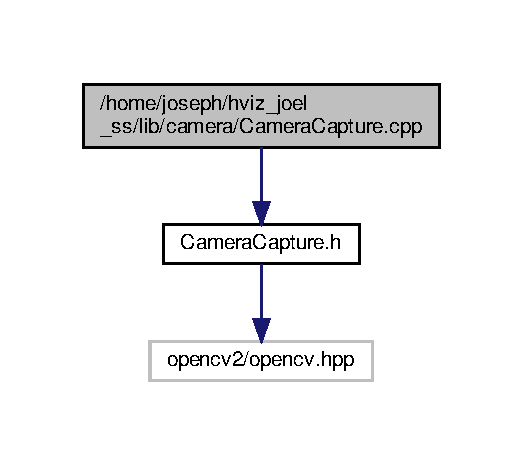
\includegraphics[width=251pt]{CameraCapture_8cpp__incl}
\end{center}
\end{figure}


\subsection{Detailed Description}
This files defines all the function needed to run the camera. 

\begin{DoxyAuthor}{Author}
Joseph Joel 
\end{DoxyAuthor}
\begin{DoxyVersion}{Version}
0.\+1 
\end{DoxyVersion}
\begin{DoxyDate}{Date}
2023-\/08-\/02
\end{DoxyDate}
\begin{DoxyCopyright}{Copyright}
Copyright (c) 2023 
\end{DoxyCopyright}

\hypertarget{CameraCapture_8h}{}\section{/home/joseph/hviz\+\_\+joel\+\_\+ss/lib/camera/\+Camera\+Capture.h File Reference}
\label{CameraCapture_8h}\index{/home/joseph/hviz\+\_\+joel\+\_\+ss/lib/camera/\+Camera\+Capture.\+h@{/home/joseph/hviz\+\_\+joel\+\_\+ss/lib/camera/\+Camera\+Capture.\+h}}


The file declares all the headers and functions for running the camera.  


{\ttfamily \#include $<$opencv2/opencv.\+hpp$>$}\newline
Include dependency graph for Camera\+Capture.\+h\+:\nopagebreak
\begin{figure}[H]
\begin{center}
\leavevmode
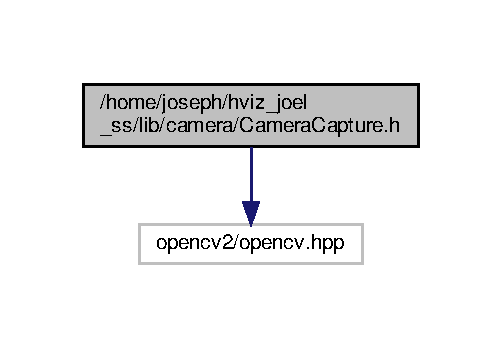
\includegraphics[width=241pt]{CameraCapture_8h__incl}
\end{center}
\end{figure}
This graph shows which files directly or indirectly include this file\+:\nopagebreak
\begin{figure}[H]
\begin{center}
\leavevmode
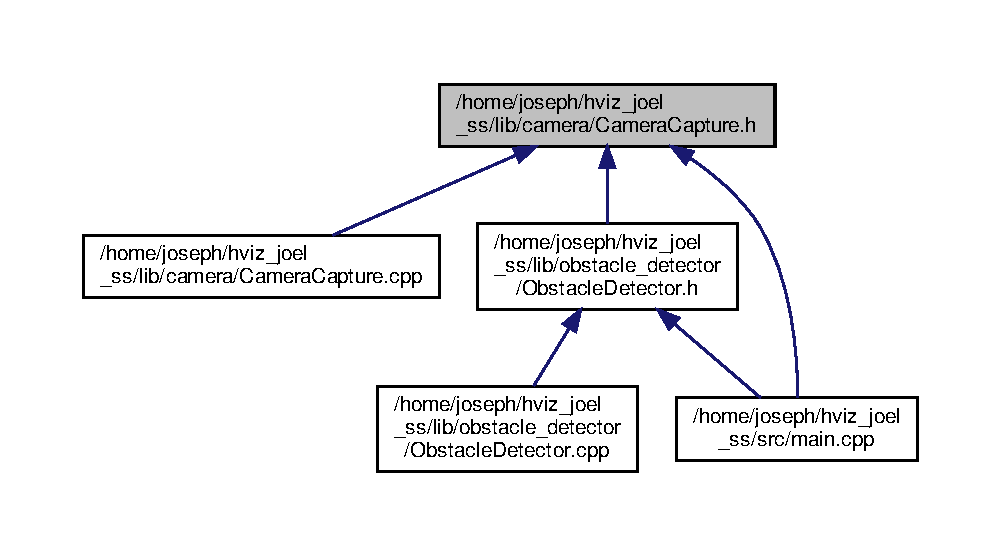
\includegraphics[width=350pt]{CameraCapture_8h__dep__incl}
\end{center}
\end{figure}
\subsection*{Classes}
\begin{DoxyCompactItemize}
\item 
class \hyperlink{classCameraCapture}{Camera\+Capture}
\end{DoxyCompactItemize}


\subsection{Detailed Description}
The file declares all the headers and functions for running the camera. 

\begin{DoxyAuthor}{Author}
Joseph Joel 
\end{DoxyAuthor}
\begin{DoxyVersion}{Version}
0.\+1 
\end{DoxyVersion}
\begin{DoxyDate}{Date}
2023-\/08-\/02
\end{DoxyDate}
\begin{DoxyCopyright}{Copyright}
Copyright (c) 2023 
\end{DoxyCopyright}

\hypertarget{GPIOController_8cpp}{}\section{/home/joseph/hviz\+\_\+joel\+\_\+ss/lib/gpio\+\_\+controller/\+G\+P\+I\+O\+Controller.cpp File Reference}
\label{GPIOController_8cpp}\index{/home/joseph/hviz\+\_\+joel\+\_\+ss/lib/gpio\+\_\+controller/\+G\+P\+I\+O\+Controller.\+cpp@{/home/joseph/hviz\+\_\+joel\+\_\+ss/lib/gpio\+\_\+controller/\+G\+P\+I\+O\+Controller.\+cpp}}


Contains all the function needed to actuate the motors on the gloves.  


{\ttfamily \#include \char`\"{}G\+P\+I\+O\+Controller.\+h\char`\"{}}\newline
Include dependency graph for G\+P\+I\+O\+Controller.\+cpp\+:\nopagebreak
\begin{figure}[H]
\begin{center}
\leavevmode
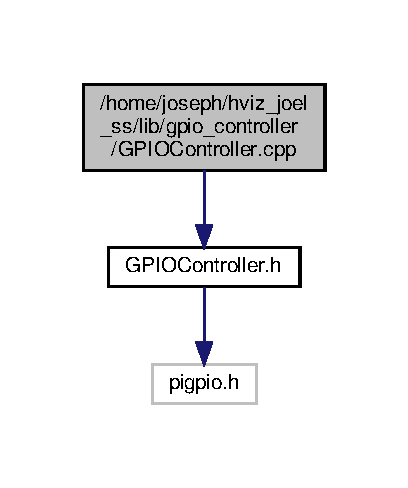
\includegraphics[width=196pt]{GPIOController_8cpp__incl}
\end{center}
\end{figure}


\subsection{Detailed Description}
Contains all the function needed to actuate the motors on the gloves. 

\begin{DoxyAuthor}{Author}
Joseph Joel 
\end{DoxyAuthor}
\begin{DoxyVersion}{Version}
0.\+1 
\end{DoxyVersion}
\begin{DoxyDate}{Date}
2023-\/08-\/02
\end{DoxyDate}
\begin{DoxyCopyright}{Copyright}
Copyright (c) 2023 
\end{DoxyCopyright}

\hypertarget{GPIOController_8h}{}\section{/home/joseph/hviz\+\_\+joel\+\_\+ss/lib/gpio\+\_\+controller/\+G\+P\+I\+O\+Controller.h File Reference}
\label{GPIOController_8h}\index{/home/joseph/hviz\+\_\+joel\+\_\+ss/lib/gpio\+\_\+controller/\+G\+P\+I\+O\+Controller.\+h@{/home/joseph/hviz\+\_\+joel\+\_\+ss/lib/gpio\+\_\+controller/\+G\+P\+I\+O\+Controller.\+h}}


The file declares all the headers and functions to actuate the motors on the gloves.  


{\ttfamily \#include $<$pigpio.\+h$>$}\newline
Include dependency graph for G\+P\+I\+O\+Controller.\+h\+:\nopagebreak
\begin{figure}[H]
\begin{center}
\leavevmode
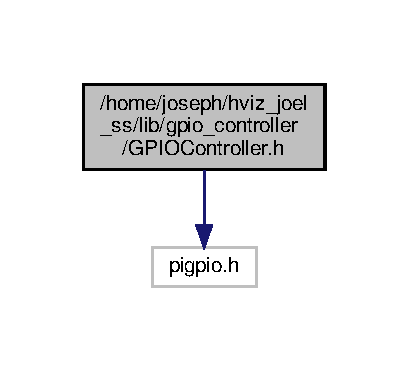
\includegraphics[width=196pt]{GPIOController_8h__incl}
\end{center}
\end{figure}
This graph shows which files directly or indirectly include this file\+:\nopagebreak
\begin{figure}[H]
\begin{center}
\leavevmode
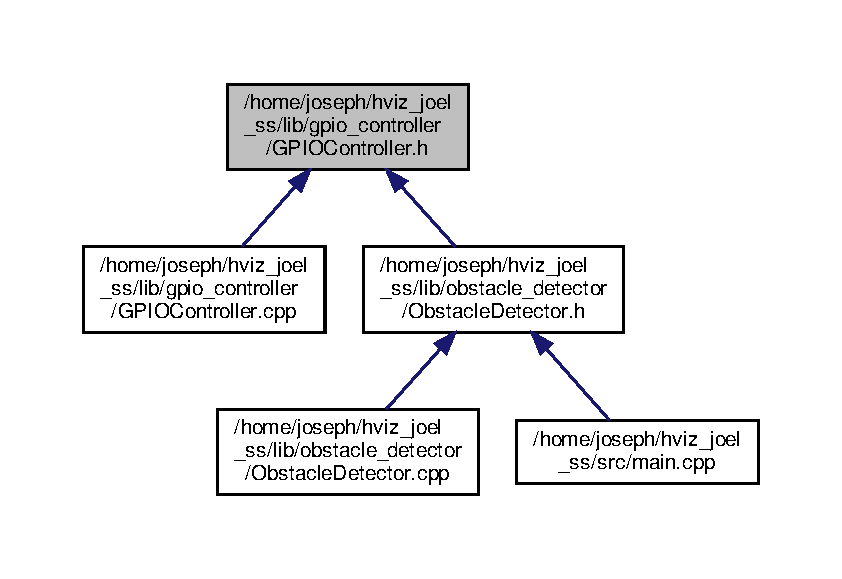
\includegraphics[width=350pt]{GPIOController_8h__dep__incl}
\end{center}
\end{figure}
\subsection*{Classes}
\begin{DoxyCompactItemize}
\item 
class \hyperlink{classGPIOController}{G\+P\+I\+O\+Controller}
\end{DoxyCompactItemize}


\subsection{Detailed Description}
The file declares all the headers and functions to actuate the motors on the gloves. 

\begin{DoxyAuthor}{Author}
Joseph Joel 
\end{DoxyAuthor}
\begin{DoxyVersion}{Version}
0.\+1 
\end{DoxyVersion}
\begin{DoxyDate}{Date}
2023-\/08-\/02
\end{DoxyDate}
\begin{DoxyCopyright}{Copyright}
Copyright (c) 2023 
\end{DoxyCopyright}

\hypertarget{ObstacleDetector_8cpp}{}\section{/home/joseph/hviz\+\_\+joel\+\_\+ss/lib/obstacle\+\_\+detector/\+Obstacle\+Detector.cpp File Reference}
\label{ObstacleDetector_8cpp}\index{/home/joseph/hviz\+\_\+joel\+\_\+ss/lib/obstacle\+\_\+detector/\+Obstacle\+Detector.\+cpp@{/home/joseph/hviz\+\_\+joel\+\_\+ss/lib/obstacle\+\_\+detector/\+Obstacle\+Detector.\+cpp}}


Code to detect and read out position of obstacle.  


{\ttfamily \#include \char`\"{}Obstacle\+Detector.\+h\char`\"{}}\newline
Include dependency graph for Obstacle\+Detector.\+cpp\+:\nopagebreak
\begin{figure}[H]
\begin{center}
\leavevmode
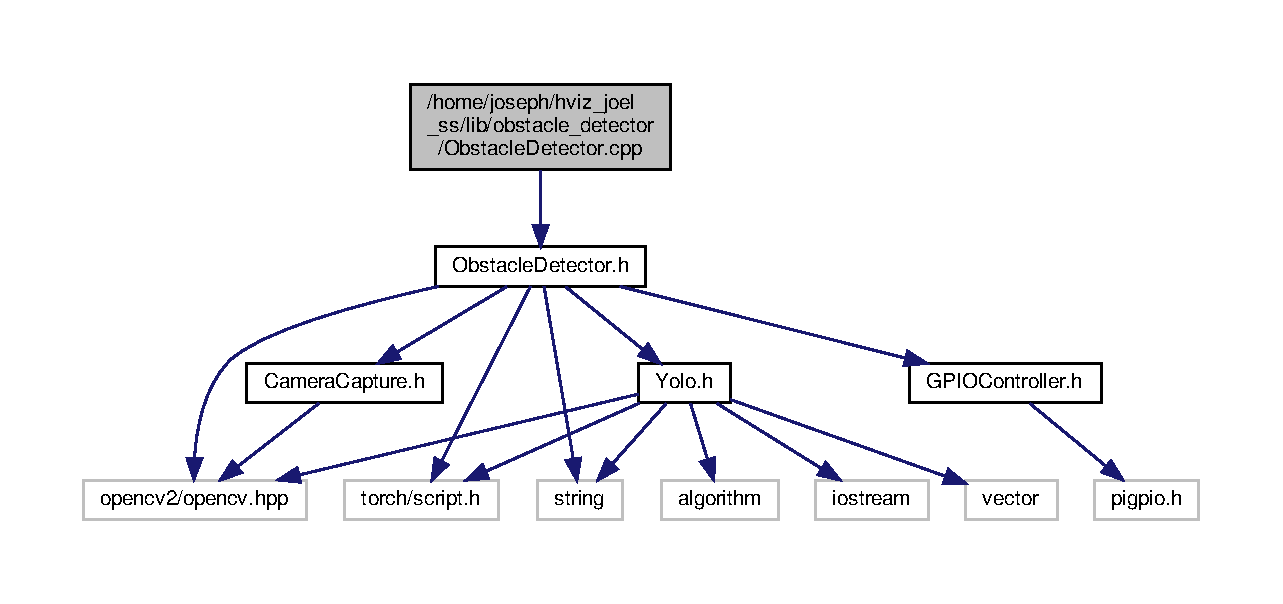
\includegraphics[width=350pt]{ObstacleDetector_8cpp__incl}
\end{center}
\end{figure}


\subsection{Detailed Description}
Code to detect and read out position of obstacle. 

\begin{DoxyAuthor}{Author}
Joseph Joel 
\end{DoxyAuthor}
\begin{DoxyVersion}{Version}
0.\+1 
\end{DoxyVersion}
\begin{DoxyDate}{Date}
2023-\/08-\/02
\end{DoxyDate}
\begin{DoxyCopyright}{Copyright}
Copyright (c) 2023 
\end{DoxyCopyright}

\hypertarget{ObstacleDetector_8h}{}\section{/home/joseph/hviz\+\_\+joel\+\_\+ss/lib/obstacle\+\_\+detector/\+Obstacle\+Detector.h File Reference}
\label{ObstacleDetector_8h}\index{/home/joseph/hviz\+\_\+joel\+\_\+ss/lib/obstacle\+\_\+detector/\+Obstacle\+Detector.\+h@{/home/joseph/hviz\+\_\+joel\+\_\+ss/lib/obstacle\+\_\+detector/\+Obstacle\+Detector.\+h}}


The file declares all the headers and functions to detct position of obstacle.  


{\ttfamily \#include $<$torch/script.\+h$>$}\newline
{\ttfamily \#include $<$opencv2/opencv.\+hpp$>$}\newline
{\ttfamily \#include $<$string$>$}\newline
{\ttfamily \#include \char`\"{}Yolo.\+h\char`\"{}}\newline
{\ttfamily \#include \char`\"{}Camera\+Capture.\+h\char`\"{}}\newline
{\ttfamily \#include \char`\"{}G\+P\+I\+O\+Controller.\+h\char`\"{}}\newline
Include dependency graph for Obstacle\+Detector.\+h\+:\nopagebreak
\begin{figure}[H]
\begin{center}
\leavevmode
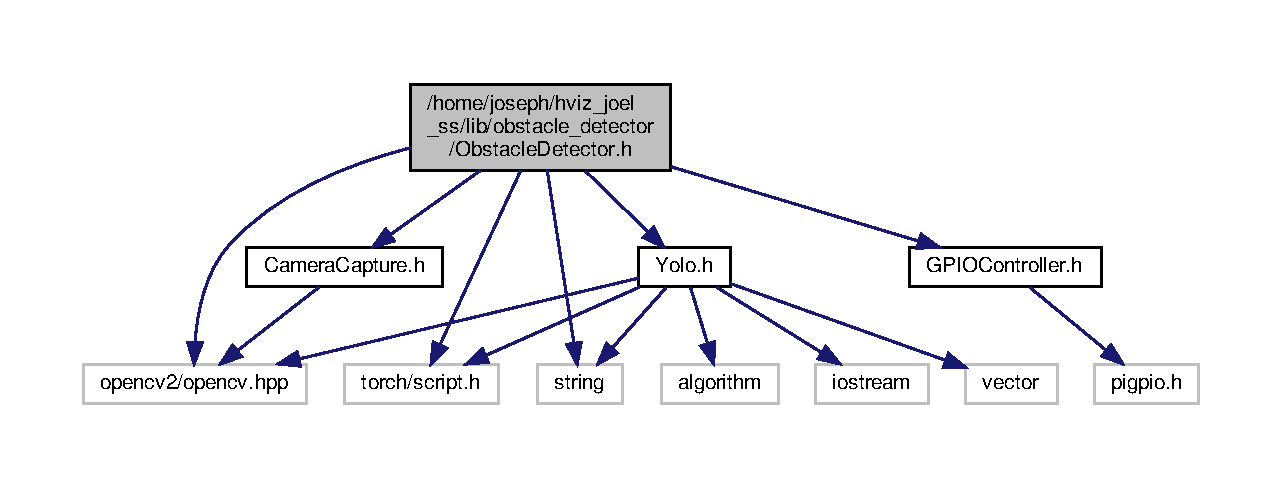
\includegraphics[width=350pt]{ObstacleDetector_8h__incl}
\end{center}
\end{figure}
This graph shows which files directly or indirectly include this file\+:\nopagebreak
\begin{figure}[H]
\begin{center}
\leavevmode
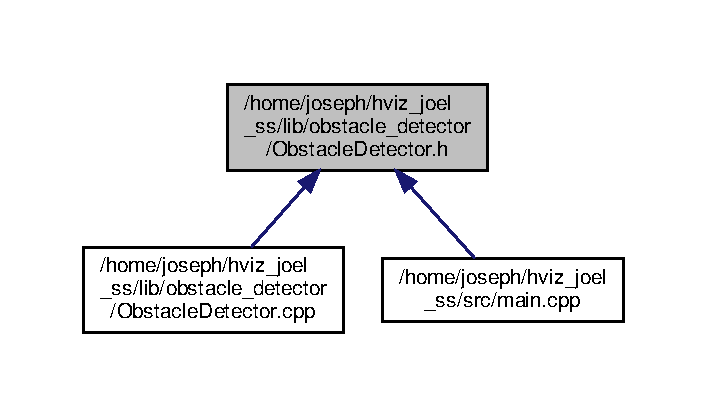
\includegraphics[width=340pt]{ObstacleDetector_8h__dep__incl}
\end{center}
\end{figure}
\subsection*{Classes}
\begin{DoxyCompactItemize}
\item 
class \hyperlink{classObstacleDetector}{Obstacle\+Detector}
\end{DoxyCompactItemize}


\subsection{Detailed Description}
The file declares all the headers and functions to detct position of obstacle. 

\begin{DoxyAuthor}{Author}
Joseph Jeol 
\end{DoxyAuthor}
\begin{DoxyVersion}{Version}
0.\+1 
\end{DoxyVersion}
\begin{DoxyDate}{Date}
2023-\/08-\/02
\end{DoxyDate}
\begin{DoxyCopyright}{Copyright}
Copyright (c) 2023 
\end{DoxyCopyright}

\hypertarget{Yolo_8cpp}{}\section{/home/joseph/hviz\+\_\+joel\+\_\+ss/lib/yolo/\+Yolo.cpp File Reference}
\label{Yolo_8cpp}\index{/home/joseph/hviz\+\_\+joel\+\_\+ss/lib/yolo/\+Yolo.\+cpp@{/home/joseph/hviz\+\_\+joel\+\_\+ss/lib/yolo/\+Yolo.\+cpp}}


Contains all the definitions of functions need for object detection using Y\+O\+LO.  


{\ttfamily \#include \char`\"{}Yolo.\+h\char`\"{}}\newline
Include dependency graph for Yolo.\+cpp\+:\nopagebreak
\begin{figure}[H]
\begin{center}
\leavevmode
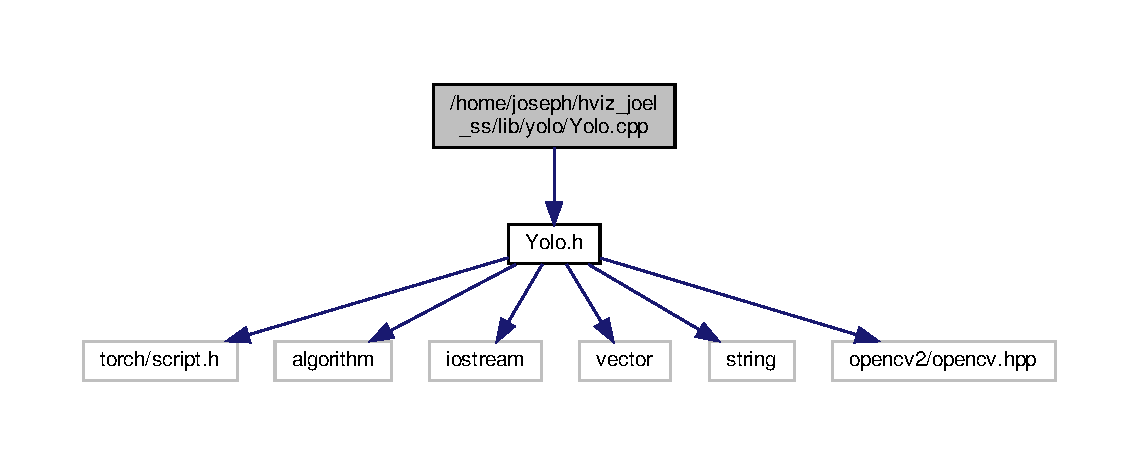
\includegraphics[width=350pt]{Yolo_8cpp__incl}
\end{center}
\end{figure}


\subsection{Detailed Description}
Contains all the definitions of functions need for object detection using Y\+O\+LO. 

\begin{DoxyAuthor}{Author}
Joseph Joel 
\end{DoxyAuthor}
\begin{DoxyVersion}{Version}
0.\+1 
\end{DoxyVersion}
\begin{DoxyDate}{Date}
2023-\/08-\/02
\end{DoxyDate}
\begin{DoxyCopyright}{Copyright}
Copyright (c) 2023 
\end{DoxyCopyright}

\hypertarget{Yolo_8h}{}\section{/home/joseph/hviz\+\_\+joel\+\_\+ss/lib/yolo/\+Yolo.h File Reference}
\label{Yolo_8h}\index{/home/joseph/hviz\+\_\+joel\+\_\+ss/lib/yolo/\+Yolo.\+h@{/home/joseph/hviz\+\_\+joel\+\_\+ss/lib/yolo/\+Yolo.\+h}}


This file declares all the headers and functions needed for Y\+O\+LO object detection and clasiffication.  


{\ttfamily \#include $<$torch/script.\+h$>$}\newline
{\ttfamily \#include $<$algorithm$>$}\newline
{\ttfamily \#include $<$iostream$>$}\newline
{\ttfamily \#include $<$vector$>$}\newline
{\ttfamily \#include $<$string$>$}\newline
{\ttfamily \#include $<$opencv2/opencv.\+hpp$>$}\newline
Include dependency graph for Yolo.\+h\+:\nopagebreak
\begin{figure}[H]
\begin{center}
\leavevmode
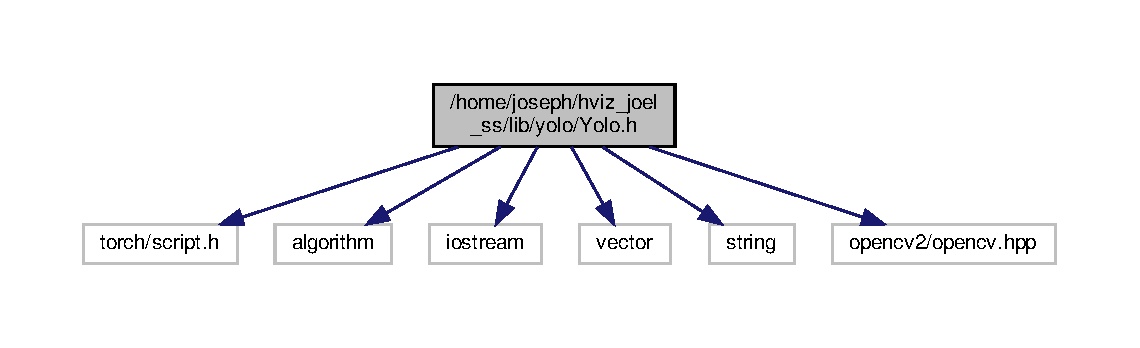
\includegraphics[width=350pt]{Yolo_8h__incl}
\end{center}
\end{figure}
This graph shows which files directly or indirectly include this file\+:\nopagebreak
\begin{figure}[H]
\begin{center}
\leavevmode
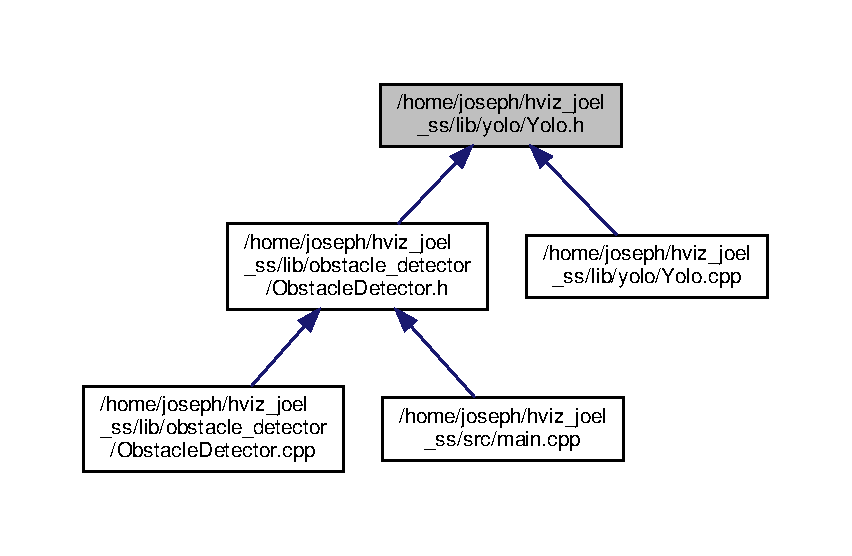
\includegraphics[width=350pt]{Yolo_8h__dep__incl}
\end{center}
\end{figure}
\subsection*{Classes}
\begin{DoxyCompactItemize}
\item 
class \hyperlink{classYolo}{Yolo}
\end{DoxyCompactItemize}


\subsection{Detailed Description}
This file declares all the headers and functions needed for Y\+O\+LO object detection and clasiffication. 

\begin{DoxyAuthor}{Author}
Joseph Joel 
\end{DoxyAuthor}
\begin{DoxyVersion}{Version}
0.\+1 
\end{DoxyVersion}
\begin{DoxyDate}{Date}
2023-\/08-\/02
\end{DoxyDate}
\begin{DoxyCopyright}{Copyright}
Copyright (c) 2023 
\end{DoxyCopyright}

\hypertarget{main_8cpp}{}\section{/home/joseph/hviz\+\_\+joel\+\_\+ss/src/main.cpp File Reference}
\label{main_8cpp}\index{/home/joseph/hviz\+\_\+joel\+\_\+ss/src/main.\+cpp@{/home/joseph/hviz\+\_\+joel\+\_\+ss/src/main.\+cpp}}


This file is the main code to run the system.  


{\ttfamily \#include $<$iostream$>$}\newline
{\ttfamily \#include $<$time.\+h$>$}\newline
{\ttfamily \#include \char`\"{}Camera\+Capture.\+h\char`\"{}}\newline
{\ttfamily \#include \char`\"{}Obstacle\+Detector.\+h\char`\"{}}\newline
Include dependency graph for main.\+cpp\+:\nopagebreak
\begin{figure}[H]
\begin{center}
\leavevmode
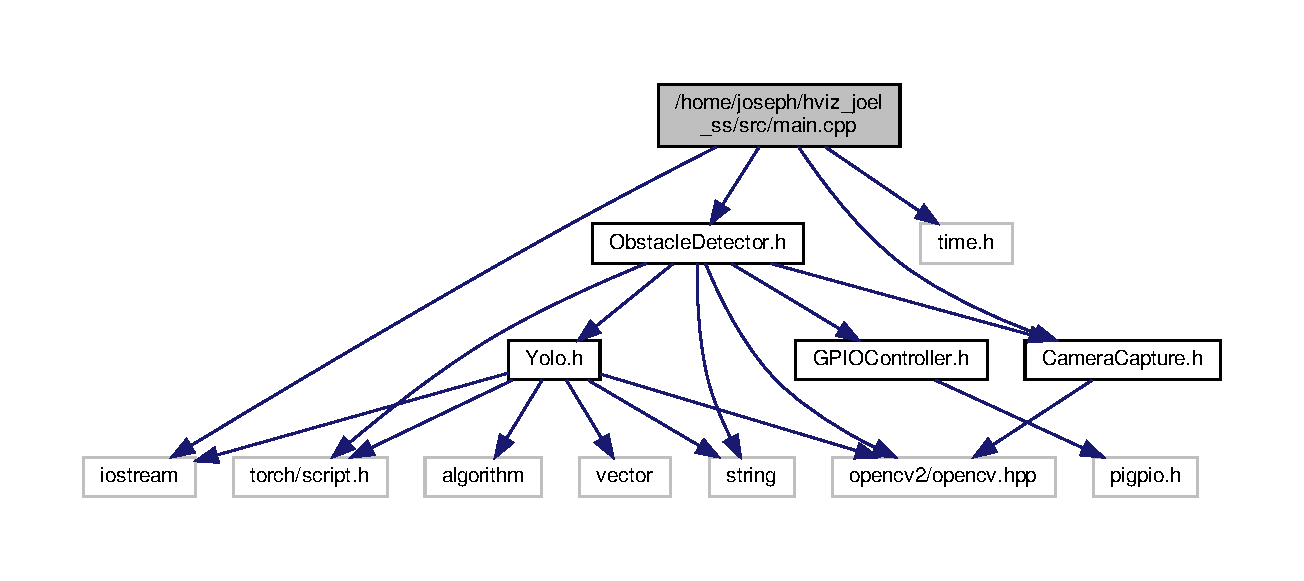
\includegraphics[width=350pt]{main_8cpp__incl}
\end{center}
\end{figure}
\subsection*{Functions}
\begin{DoxyCompactItemize}
\item 
int \hyperlink{main_8cpp_ae66f6b31b5ad750f1fe042a706a4e3d4}{main} ()
\begin{DoxyCompactList}\small\item\em This is the main function to the run the system. \end{DoxyCompactList}\end{DoxyCompactItemize}


\subsection{Detailed Description}
This file is the main code to run the system. 

\begin{DoxyAuthor}{Author}
Joseph Joel 
\end{DoxyAuthor}
\begin{DoxyVersion}{Version}
0.\+1 
\end{DoxyVersion}
\begin{DoxyDate}{Date}
2023-\/08-\/02
\end{DoxyDate}
\begin{DoxyCopyright}{Copyright}
Copyright (c) 2023 
\end{DoxyCopyright}


\subsection{Function Documentation}
\mbox{\Hypertarget{main_8cpp_ae66f6b31b5ad750f1fe042a706a4e3d4}\label{main_8cpp_ae66f6b31b5ad750f1fe042a706a4e3d4}} 
\index{main.\+cpp@{main.\+cpp}!main@{main}}
\index{main@{main}!main.\+cpp@{main.\+cpp}}
\subsubsection{\texorpdfstring{main()}{main()}}
{\footnotesize\ttfamily int main (\begin{DoxyParamCaption}{ }\end{DoxyParamCaption})}



This is the main function to the run the system. 

\begin{DoxyReturn}{Returns}
int 
\end{DoxyReturn}

%--- End generated contents ---

% Index
\backmatter
\newpage
\phantomsection
\clearemptydoublepage
\addcontentsline{toc}{chapter}{Index}
\printindex

\end{document}
